\section{Déploiement}
\subsection{Étude de marché}
\subsubsection{Avant-propos}
Il existe de nos jours une multitude de solutions afin d'héberger une application web. Toutes les solutions offrent divers avantages et inconvénients, aussi bien d'un point de vue technologique que financier. Afin de ne pas s'encombrer avec une quantité importante de possibilités, j'ai sélectionné quatre options qui me paraissent les plus adéquates :
\begin{itemize}
  \item Serveur local
  \item Heroku (\textit{\url{https://www.heroku.com/home}})
  \item Microsoft Azure (\textit{\url{https://azure.microsoft.com/en-us/}})
  \item Virtual Private Server (VPS) chez OVH (\textit{\url{https://www.ovhcloud.com/fr/vps/}})
\end{itemize}

\newpara

Dans le cadre de ce projet, il est important de préciser les contraintes suivantes :
\begin{itemize}
  \item le client n'a \textbf{pas d'informaticien} à temps plein
  \item le client souhaite \textbf{limiter les dépenses} au maximum
  \item le \textbf{trafic} vers l'application sera \textbf{faible} car utilisé uniquement par une ou deux personnes et pendant 2-3h par jour maximum
  \item dans le futur, un web-shop pourrait être intégré à l'application et donc générer un trafic plus important -> \textbf{évolutivité}
\end{itemize}

\newpara

La solution doit pouvoir :
\begin{itemize}
  \item Héberger une application NodeJs
  \item Héberger une base de données SQL
\end{itemize}
(Idéalement les deux services sont hébergés sur la même plateforme mais ce n'est pas obligatoire.)

\newpage
\subsubsection{Étude des solutions}
\subsubsubsection{Serveur Local} 

\textbf{Description}: \\ Le client utilise actuellement un serveur tournant sous Windows 10 pro. Ce serveur, situé dans l'atelier mécanique, fait tourner leur programme de gestion mais sert également d'ordinateur "classique" pour tous les employés. Notons qu'aucun système de backup automatique n'est mis en place. La base de données inclue dans leur programme de gestion devant être aussi accessible depuis le site de la carrosserie, une règle de port-forwarding est mise en place dans le firewall de leur routeur.

\newpara
\textbf{Avantages}:
\begin{itemize}
  \item Coût négligeable car infrastructure existante
  \item Maîtrise totale des données
\end{itemize}

\newpara
\textbf{Inconvénients}:
\begin{itemize}
  \item OS du serveur inadapté (Windows 10 pro)
  \item Maintenance plus compliquée à mettre en place
  \item "Scalabilité"\footnote{Capacité de s'adapter en fonction de la charge (trafic réseau, puissance de calcul, ...)} compliquée voir impossible sans investissement conséquent
  \item Déploiement continu plus complexe à mettre en place
  \item Accessibilité extérieure requière plus de sécurité
  \item Nécessite la mise en place d'une meilleur gestion des backups
  \item Pas de redondance
\end{itemize}

\newpara
\textbf{Prix}: \\ L'infrastructure physique déjà existante et l'utilisation de software gratuit et open-source tels qu'Apache, PostgreSql, fail2ban,... rendraient les coûts négligeables.

\newpara
\textbf{Coût estimé en production}: ±0 €/mois

\newpara
\textbf{Conclusion} \\ Au vu des nombreux désavantages, je pense que cette solution, bien que peu coûteuse, ne soit pas envisageable.

\newpage
\subsubsubsection{Heroku}

\textbf{Description}: \\ Heroku est un PaaS(Platform as a Service) fortement utilisé de par sa simplicité et sa compatibilité avec des languages modernes tels que Node, Ruby, Python et bien d'autres.
\newpara
Bien que souvent utilisé pour des projets de petite à moyenne taille, certaines grandes entreprises comme Toyota Europe ou Dubsmash l'utilisent également.

\newpara
\textbf{Avantages}:
\begin{itemize}
  \item Intégration très facile avec "Git"
  \item Entièrement gratuite pour le développement
  \item Inclus une base de données PostgreSql
  \item Coût en production fixe
  \item Maintenance facile et accessible à distance
  \item Portabilité élevée: il est très facile d'arrêter le service et de migrer vers une autre solution. Le code n'est pas lié à Heroku
  \item Expérience: j'ai déjà plusieurs fois eu l'occasion de travailler avec Heroku, je connais assez bien la plateforme et la façon de travailler avec celle-ci
  \item Métriques inclus
  \item Sécurité  
\end{itemize}

\newpara
\textbf{Inconvénients}:
\begin{itemize}
  \item "Scalabilité" moyenne car il faut changer de plan tarifaire en fonction du trafic
  \item Gestion de la base de données moins facile (pas de rôles différents)
  \item Cold-starts d'une à deux minutes du site-web (uniquement avec la version gratuite)
\end{itemize}

\newpara
\textbf{Prix}: \\ Heroku fonctionne sur base de plans tarifaires prédéfinis mais modulables. En fonction des besoins du client, j'ai sélectionné 4 plans tarifaires:
\begin{itemize}
  \newpage
  \item \textbf{Hobby - gratuit}: \\ Ce plan tarifaire offre pratiquement toutes les fonctionnalités dont nous avons besoin. Nous serons néanmoins restreints par le nombre de requêtes, la taille de la base de données, les cold-starts, ... Cette solution me semble plus que suffisante durant le développement de l'application et pourquoi pas durant les premiers mois ou premières années d'utilisation. Attention, la DB gratuite est limitée à $10^4$ lignes.
  \begin{figure}[H]
    \centering
    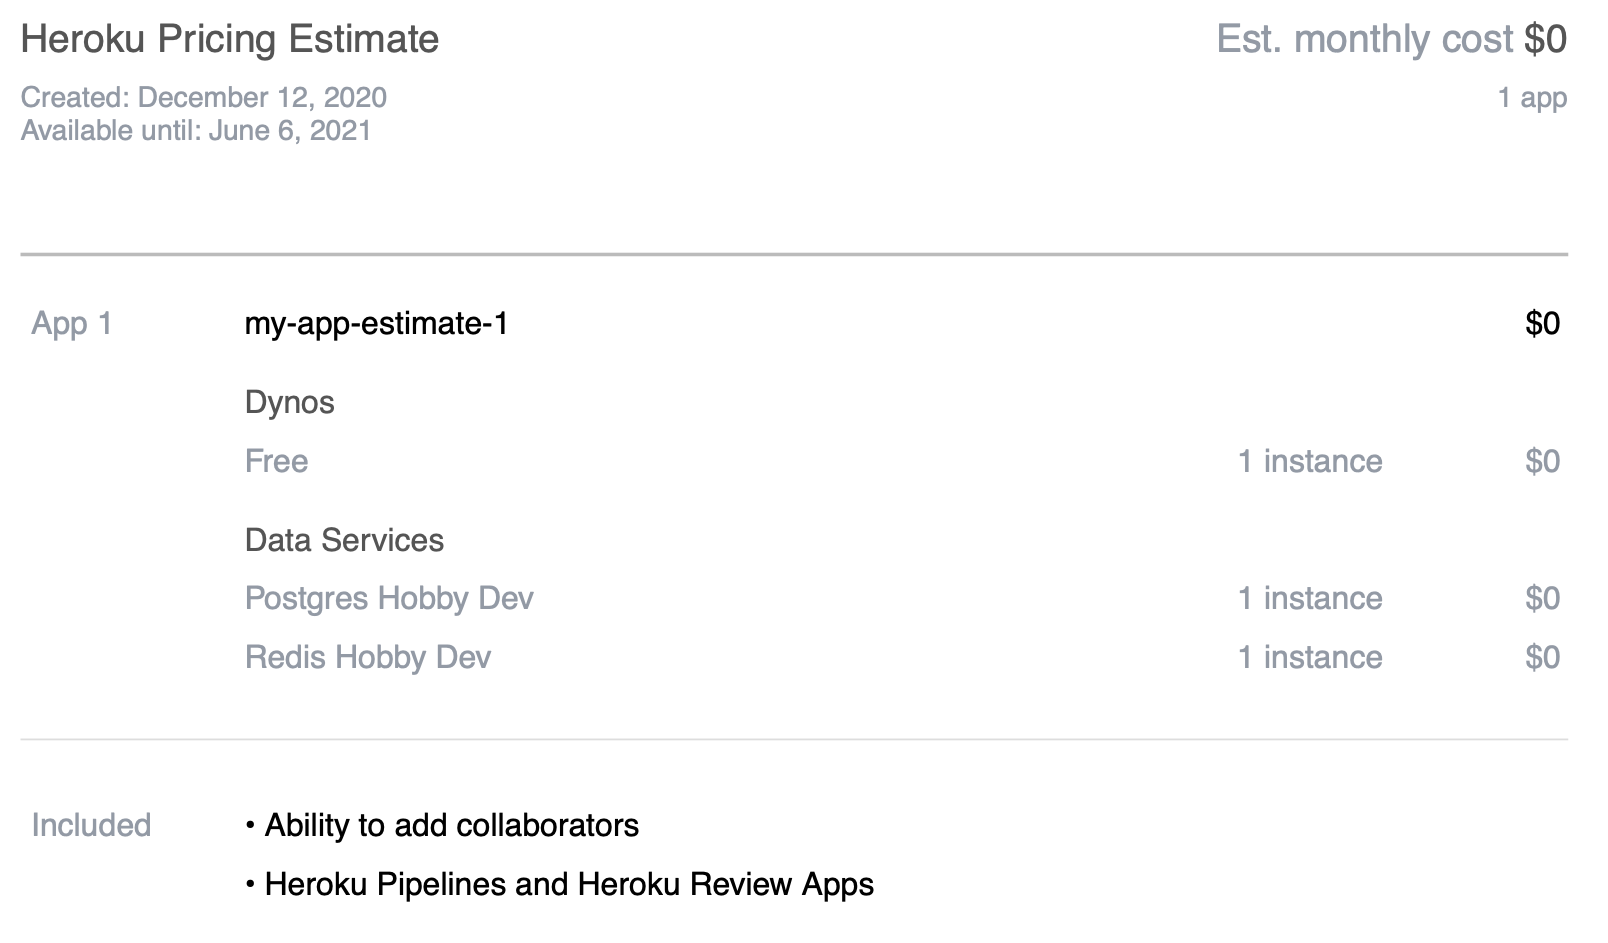
\includegraphics[width=0.75\linewidth]{img/heroku/Heroku_free.png}
  \end{figure}

  \item \textbf{Hobby - basic}: \\ Ce plan tarifaire est identique au précédent sauf que la DB peut accueillir $10^7$ lignes.
  \begin{figure}[H]
    \centering
    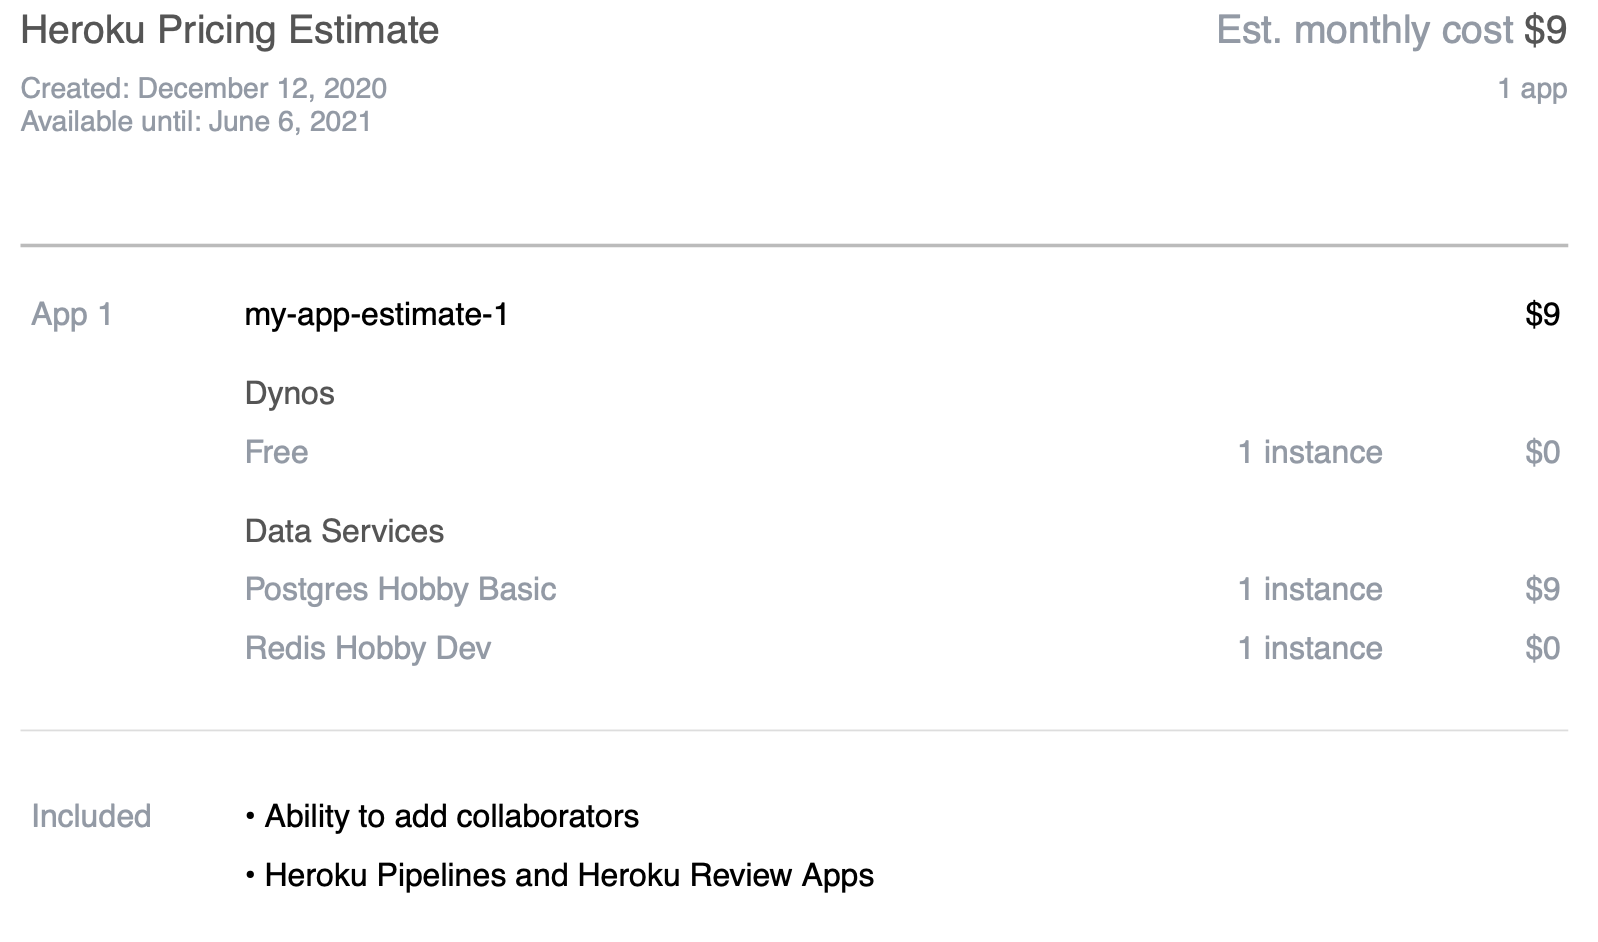
\includegraphics[width=0.75\linewidth]{img/heroku/Heroku_basic.png}
  \end{figure}
  
  \newpage
  \item \textbf{Hobby - avancé}: \\ Ce plan tarifaire est à peu de chose prêt équivalent au plan "basic". Il permet néanmoins de supprimer complètement les cold-starts. Il offre également les métriques du site pour les dernières 24h.
  \begin{figure}[H]
    \centering
    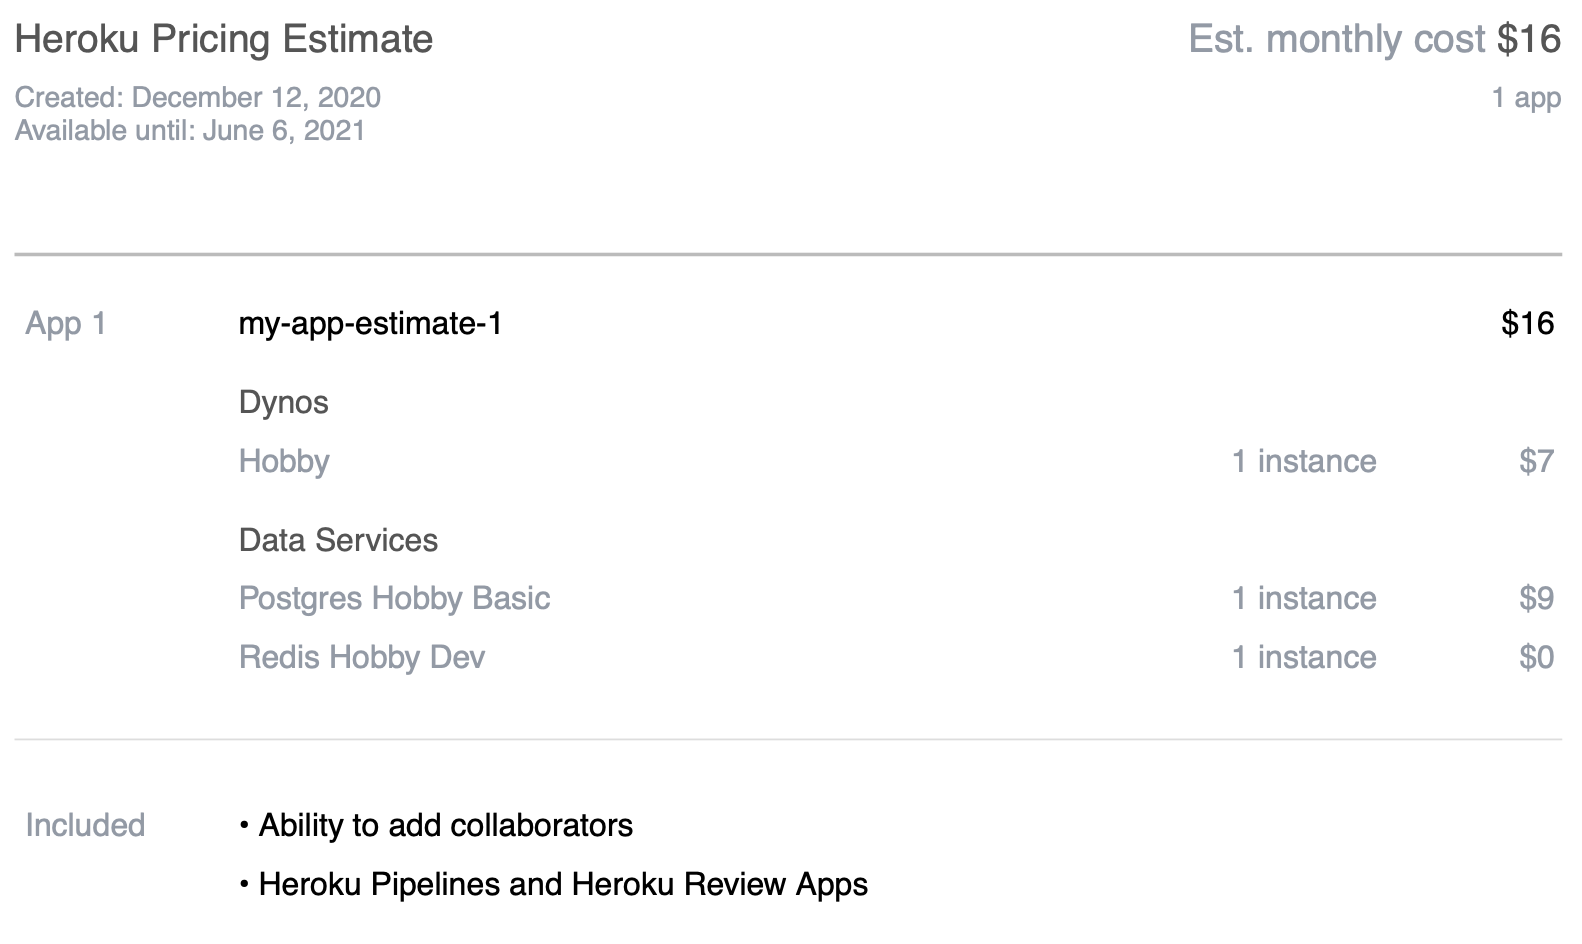
\includegraphics[width=0.75\linewidth]{img/heroku/Heroku_hobby.png}
  \end{figure}
  
  \item \textbf{Production}: \\ Ce plan offre tout ce que les plans précédents offrent mais augmente considérablement les capacité de gestion de trafic, augmente la taille maximale de la base de données, offre des métriques détaillées aussi bien pour la base de données que pour le site-web et permet des roll-backs sur une période de 7 jours.
  \begin{figure}[H]
    \centering
    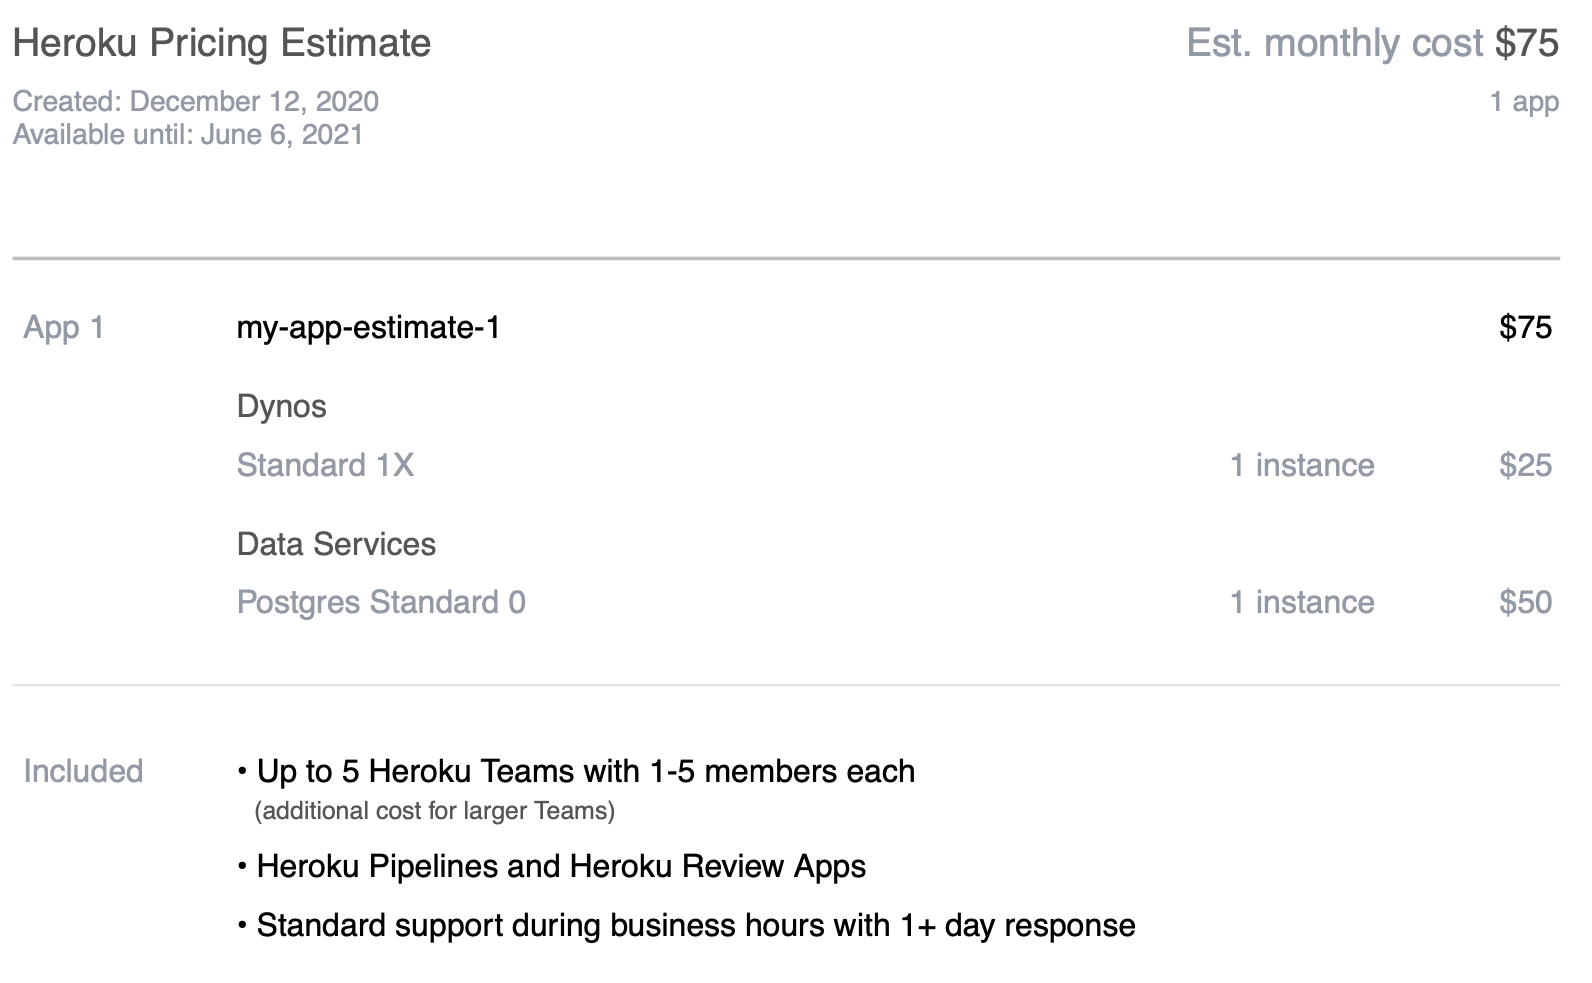
\includegraphics[width=0.75\linewidth]{img/heroku/Heroku_prod.png}
  \end{figure}
\end{itemize}

\newpage
\textbf{Conclusion} \\ Sur base de ces options, je pense qu'il est possible de partir dans un premier temps sur le plan tarifaire n°2. Néanmoins le jour où le client souhaite ajouter un web-shop à l'application, il faudra probablement passer sur un autre plan tarifaire tel que le n°3.
\newpara
En plus du coût du plan n°2, il est bon de prendre une petite marge de sécurité afin de ne pas être surpris par d'éventuels coûts supplémentaires tels qu'un nom de domaine, un autre certificat SSL,...

\newpara
\textbf{Coût estimé en production}: 18 €/mois

\newpage
\subsubsubsection{Microsoft Azure}

\textbf{Description}: \\ Microsoft Azure est un des leaders dans le domaine des cloud service providers. La plateforme offre plus de 200 produits couvrant une multitude de domaines allant de la location de ressources de calculs pour du "Machine Learning" à l'hébergement de base de données en passant par la gestion de conteneurs Docker.
\newpara
Microsoft Azure est utilisé par un très grand nombre d'entreprises tel que 3M, Airbus, Avid, BMW et bien d'autres.

\newpara
\textbf{Avantages}:
\begin{itemize}
  \item Scalabilité extrêmement performante
  \item Compartimentation de chaque service
  \item Documentation et communauté très actives
  \item Grande flexibilité de configuration
  \item Maintenance facile et accessible à distance
  \item Métriques inclus
  \item Sécurité
\end{itemize}

\newpara
\textbf{Inconvénients}:
\begin{itemize}
  \item Coût très variable et difficile à prévoir à l'avance
  \item Complexe à configurer correctement
  \item Je n'ai aucune expérience
\end{itemize}

\newpara
\textbf{Prix}: \\ A l'inverse de Heroku, Azure ne fonctionne pas sur base de plans tarifaires spécifiques mais bien sur base du principe "Pay-as-you-go". Le coût dépend donc fortement du trafic, de la taille de la base de données, de la taille des requêtes etc.

\begin{itemize}
  \item \textbf{Service Web}: Hébergement de l'application sur une machine Linux :
  \begin{itemize}
    \item version gratuite pendant 12 mois
    \item version payante : 11,081€/mois
  \end{itemize}
  \item \textbf{base de données}:
  \begin{itemize}
    \item 5GB (5GB étant le minimum configurable) d'espace de stockage à 0,1155€/GB/mois soit : ±0,58€/mois
    \item 1 vCore à 0,4840€/heure: si utilisation 2h/j -> 60h/mois soit : ±29€/mois
  \end{itemize}
\end{itemize}

\newpara
\textbf{Coût estimé en production}: ±41 €/mois

\newpara
\textbf{Conclusion} \\ Bien que Microsoft Azure offre une très grande flexibilité et un environnement très professionnel, le coût semble fort élevé et pas très compétitif pour une application de cette envergure. Néanmoins, le jour où un web-shop est ajouté par le client, cette solution peut être retenue!

\newpage
\subsubsubsection{VPS OVH}

\textbf{Description}: \\ Qu'est ce qu'un VPS? \textit{"Un serveur privé virtuel est un environnement isolé, créé sur un serveur physique à partir d’une technologie de virtualisation. Cette solution offre tous les avantages d’un serveur standard, profitant de ressources allouées et d’une administration complète."}\cite{VPS}

\newpara
Il existe plusieurs entreprises de Cloud Computing offrant des services VPS tel que AWS, IBM et OVH. Ayant eu de bons échos d'OVH et ayant déjà travaillé avec leurs services, j'ai choisi de limiter ma recherche d'offre à OVH.

\newpara
\textbf{Avantages}:
\begin{itemize}
  \item Maîtrise totale des données
  \item Facile à mettre en place
  \item Grandes flexibilité de configuration
  \item Maintenance facile et accessible à distance
  \item "Scalabilité" compliquée 
  \item Métriques inclus
\end{itemize}
  
\newpara
\textbf{Inconvénients}:
\begin{itemize}
  \item Nécessite la mise en place de la sécurité du VPS
  \item Nécessite la mise en place d'une gestion des backups
  \item Redondance plus compliqué à mettre en place
\end{itemize}

\newpara
\textbf{Prix}: \\ OVH propose une multitude de plans tarifaires pour leurs VPS (voir \textit{figure \ref{ovh-pricing}} ci-dessous). Notre application étant réservée à un usage interne, le trafic généré sera faible. Le plan tarifaire le moins cher nous sera dès lors plus que suffisant. De plus il est toujours possible de changer de plan par la suite. 
\begin{figure}[H]
  \centering
  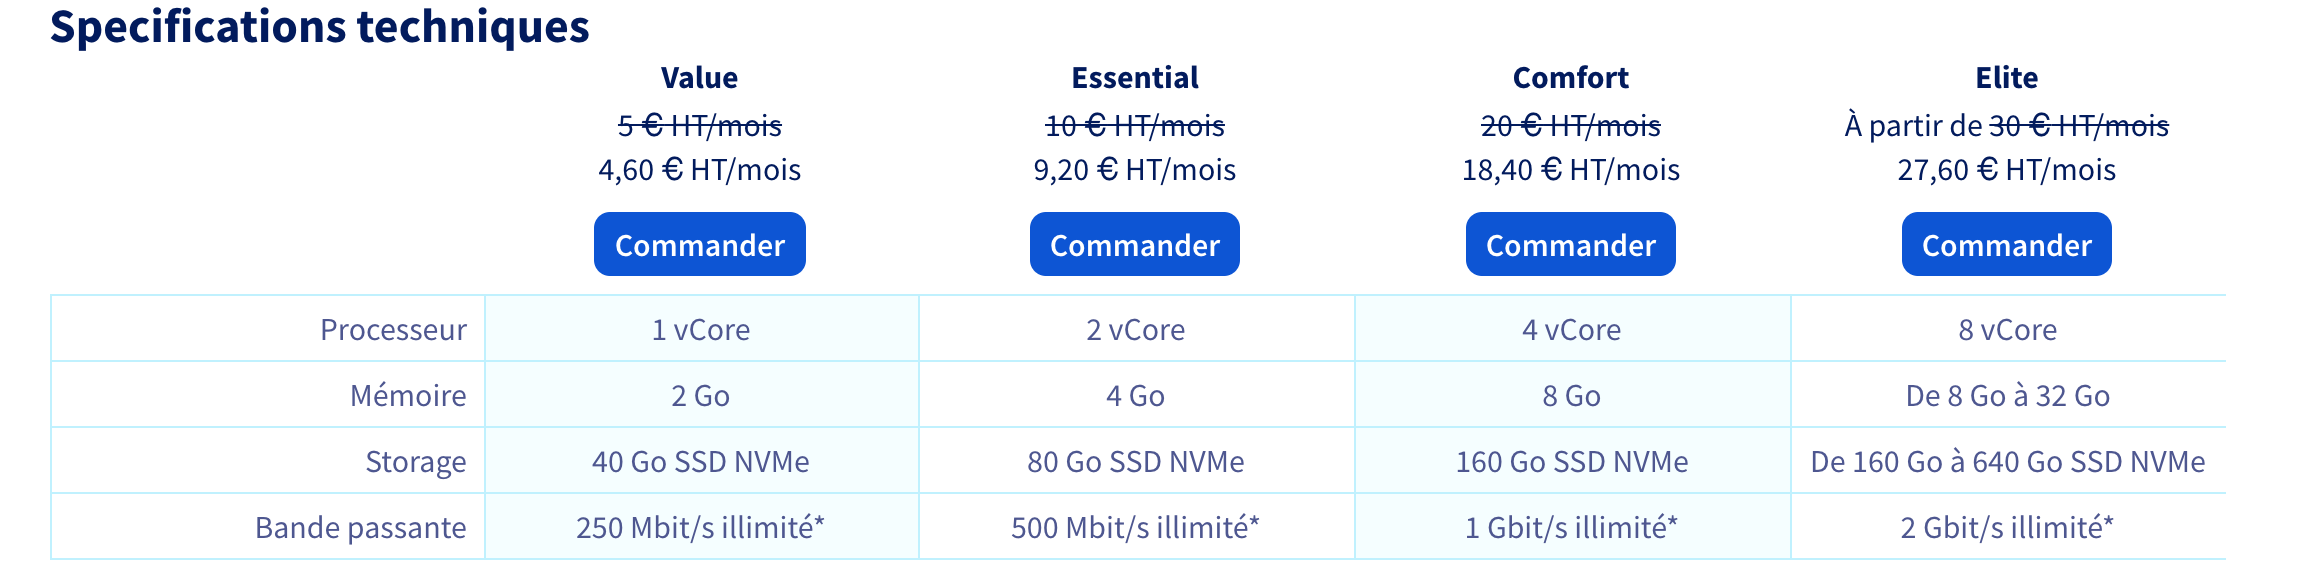
\includegraphics[width=\linewidth]{img/vps-tarifs.png}
  \caption{Tarifs VPS OVH}
  \label{ovh-pricing}
\end{figure}



\newpara
\textbf{Coût estimé en production}: ±5 €/mois

\newpara
\textbf{Conclusion} \\ Cette solution offre pratiquement tous les avantages d'un serveur local sans devoir se soucier de l'aspect hardware et ce à un prix très raisonnable. 

\newpage
\subsection{Première approche - Heroku}
Dans un but de réduire au maximum les coûts et de simplifier les choses durant le développement de l'application, le client et moi même avons décidé de déployer, dans un premier temps, celle-ci sur Heroku avec le plan gratuit. Cette solution fut plus que suffisante pendant les trois premiers mois du développement. Néanmoins, une fois l'application plus complète, plusieurs facteurs tels que: 
\begin{itemize}
  \item la lenteur de mise en production (temps nécessaire entre l'action de déploiement et l'accessibilité du site)
  \item le maximum de $10^4$ lignes dans la base de données 
\end{itemize}
nous ont fait revoir les solutions de déploiement. 

\subsection{Seconde approche - VPS}
Pour les raisons précédemment abordées, nous avons décidé de migrer l'application hébergée sur Heroku vers un VPS chez OVH. Ceci nous a permis de nous affranchir totalement des contraintes liées à la base de données mais impliquait une plus grande configuration initiale. 

\newpara

En sachant que l'application pouvait potentiellement encore être migrée dans le future, j'ai mis en place une multitude d'élements afin de rendre ces transitions les plus simples possibles. Ainsi l'entièreté de l'application est conteneurisée\footnote{\textit{"La conteneurisation informatique permet de packager tous les services, scripts, API, librairies dont une application a besoin. L’objectif : en permettre l’exécution sur n’importe quel noyau compatible."}\cite{conteneurisation}} et toutes les configurations du VPS sont scriptées au maximum. 

\subsubsection{Dockerisation}
Dans le but de faciliter la configuration des différents services nécessaires au bon fonctionnement de l'application, j'ai placé chacun d'eux dans un conteneur docker. Ainsi l'application est composée de 3 conteneurs distincts: 

\newpara

\begin{enumerate}
  \item \textbf{slg-db}: La base de données PostgreSql. Port exposé: \textbf{5434}.
  \item \textbf{slg-app}: L'application NodeJs\footnote{NodeJs est un environnement d'exécution open-srouce et multi-platforme permettant de faire tourner du code Javascript.} en tant que telle, composée du backend et frontend. Port exposé \textbf{8080}. 
  \item \textbf{caddy}: Serveur web Caddy\footnote{\url{https://caddyserver.com}} utilisé en tant que reverse-proxy\footnote{Un reverse-proxy est un intermédiaire de communication réseau permettant de transmettre une requête au serveur cible en fonction du nom de domaine de cette requête.} et gestionnaire des certificats https. Ports exposés: \textbf{80} et \textbf{441}.
\end{enumerate}

\newpage

Ces trois conteneurs fonctionnent en symbiose et sont dépendants les uns des autres. Aisni, l'application node ne démarrera pas si la base de données n'a pas démarré avec succès. Afin de contrôler l'environnement dans lequel ces conteneurs sont lancés ainsi que pouvoir facilement les démarrer/arrêter, j'ai créé un fichier docker-compose\footnote{docker-compose permet d'orchestrer un ensemble de conteneurs dans le but de simplifier la gestion et la communication de ceux-ci.}. \\ (Voir: \url{https://github.com/MMichotte/SLG_APP/blob/master/docker/docker-compose.yml})

\subsubsection{Scripts}
\label{scritps}
J'ai principalement écrit 2 scripts. \textbf{Le premier} plus consistant me permet de configurer automatiquement un nouveau VPS. En pratique, celui ci exécute: 
\begin{enumerate}
  \item Mise à jour des packages
  \item Mise à jour de la time-zone
  \item Création d'un nouvel utilisateur
  \item Modification des paramètres de connexion SSH
  \item Configuration et activation de Fail2ban\footnote{Fail2ban est un programme de prévention permettant de bloquer les tentatives d'intrusion frauduleuses}
  \item Installation de docker-compose
\end{enumerate}

\newpara

\textbf{Le second} script est bien moins complexe et permet de configurer et démarrer le backup (local) journalier de la base de données. Ces backups sont réalisés périodiquement à l'aide de "crontab"\footnote{\textit{"Crontab est un outil qui permet de lancer des applications de façon régulière, pratique pour un serveur pour y lancer des scripts de sauvegardes, etc."}\cite{CRON}}.

\newpara

Il s'avère que ces scripts m'ont été très rapidement utiles. En effet, seulement 6h après la configuration complète du VPS, un incendie a ravagé plusieurs data-centers chez OVH et a détruit, entre autres, notre VPS.\footnote{Plus d'information sur l'incident: \url{https://www.ovh.com/fr/news/presse/cpl1785.dernieres-informations-notre-site-strasbourg}} Après quelques jours d'inaccessibilité, j'ai pu re-configurer un VPS dans un autre data-center. Cette re-configuration n'a pas duré plus de 10 minutes.

\newpage

\subsubsection{Sécurité}
\subsubsubsection{SSH}
\newparasm
Une connexion SSH avec le VPS est indispensable pour pouvoir le configurer et y configurer les différents services. Cependant c'est aussi une des principales portes d'entrée pour les personnes malveillantes. Afin de réduire au maximum les risques, j'ai configuré le service SSH de telle sorte que :
\begin{itemize}
  \item il soit disponible sur le port 62222 et non 22. Un grand nombre d'attaques par force brute se basent sur le fait que par défaut le port utilisé par SSH est le 22. Dès lors changer le port par défaut permet d'éviter toute une série d'attaques automatisées. 
  \item il interdise la connexion par mot de passe. Il est désormais uniquement possible de se connecter par paire de clés SSH.
  \item il interdise la connexion en tant que root. 
\end{itemize} 

\subsubsubsection{Fail2ban}
\newparasm
Qu'est ce que Fail2ban? \textit{"fail2ban est une application qui analyse les logs de divers services (SSH, Apache, FTP…) en cherchant des correspondances entre des motifs définis dans ses filtres et les entrées des logs. Lorsqu'une correspondance est trouvée une ou plusieurs actions sont exécutées. Typiquement, fail2ban cherche des tentatives répétées de connexions infructueuses dans les fichiers journaux et procède à un bannissement en ajoutant une règle au pare-feu iptables ou nftables pour bannir l'adresse IP de la source."}\cite{F2B}

\newpara

Comme expliqué précédemment, un des points d'entrées les plus vulnérables est le service SSH. Dans le but de renforcer son imperméabilité, j'ai ajouté une règle Fail2ban limitant le nombre de tentatives de connexion à 6. Après 6 connexions échouées, l'adresse IP source est bloquée pour une durée de 1h. La durée d'un ban augmente de manière exponentielle si la même IP re-tente une multitude de connexions après s'être faite bannir. 

\newpage

\subsubsubsection{Firewall (UFW)}
\newparasm
\begin{minipage}{.5\textwidth}
  Afin de pouvoir contrôler le flux d'informations circulant entre le VPS et le réseau internet j'ai mis en place un firewall sur le VPS. Celui-ci intégrant par défaut les iptables\footnotemark, j'ai choisi d'utiliser "UFW" car celui-ci s'intègre parfaitement avec les iptables.  
\end{minipage}
\begin{minipage}{.5\textwidth}
  \begin{figure}[H]
    \centering
    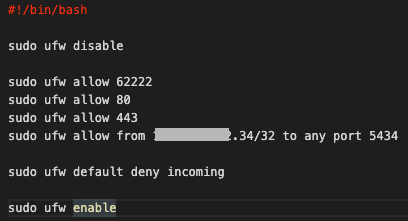
\includegraphics[width=0.8\linewidth]{img/ufw-script.png}
    \caption{Script d'ajout règles UFW}
  \end{figure}
\end{minipage}


\subsubsubsection{Firewall (OVH)}
\newparasm
En plus du firewall interne au VPS, OVH met à disposition un firewall en amont du VPS. J'ai configuré celui-ci afin d'être le plus restrictif possible (voir \textit{figure \ref{VPS-firewall}}).
\begin{figure}[H]
  \centering
  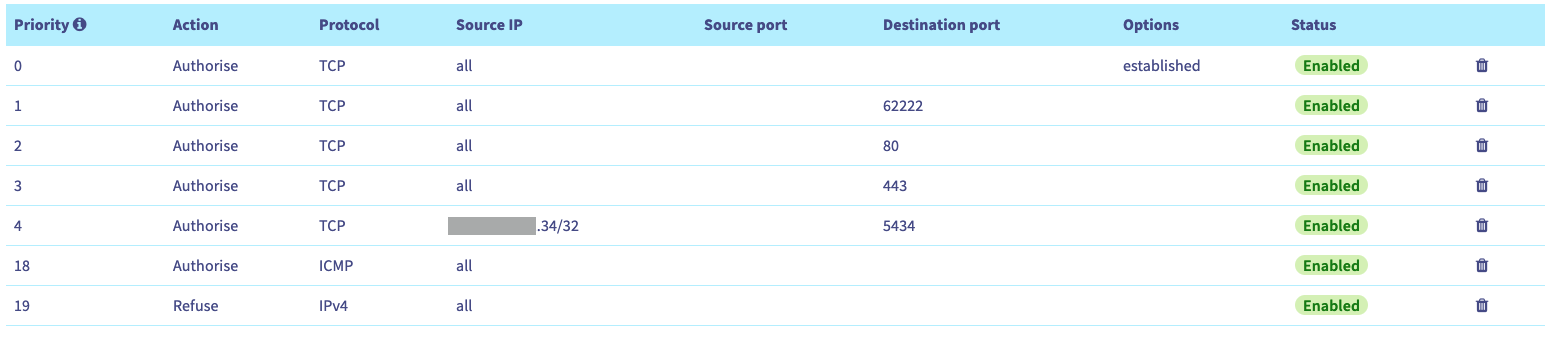
\includegraphics[width=\linewidth]{img/ovh-fireWall.png}
  \caption{Configuration du firewall en amont du VPS}
  \label{VPS-firewall}
\end{figure}

\newpara
\newpara

Notons que dans les deux firewall (UFW et OVH) le port 5434 est ouvert, ce port est utilisé par la base de données. Rendre ce port accessible publiquement est potentiellement une faille de sécurité. Néanmoins j'ai restreint l'accès à ce port à une seule adresse IP spécifique (la mienne en l'occurrence). Une fois l'application terminée, cette règle sera supprimée rendant la base de données totalement inaccessible depuis l'extérieur. 


\footnotetext{iptables est le pare-feu installé par défaut sur les système d'exploitation Linux.}

\newpage
\subsection{Intégration et Déploiement Continu (CI/CD)}

La méthodologie Agile se basant sur une succession de "sprints" aboutissant à chaque fois à une nouvelle fonctionnalité, il est important que celle-ci puisse rapidement être testée par le client afin d'en avoir un feedback et de pouvoir y apporter ou non des modifications. 

\newpara
Dans ces conditions, il est indispensable d'avoir un système d'intégration et de déploiement continu. L'intégration continue consiste à automatiser les phases de tests tandis que le déploiement continu permet d'automatiser la mise en production de la nouvelle fonctionnalité. 

\newpara
Le code de ce projet étant hébergé sur Github, j'ai pu profiter des "Github Actions"\footnote{Plus d'informations voir: \url{https://github.com/features/actions}} permettant de définir un ensemble d'actions à éxécuter sur le code et ce sur base de certaines conditions et dans un environnement isolé. Pour ce projet j'ai dès lors défini le workflow suivant :
\linebreak \linebreak
Lors d'une modification du code sur la branche "master": \\
\textbf{1.} lancement en simultané des tests unitaires frontend et backend \\
Si tous les tests sont passés avec succès: \\
\textbf{2.} déploiement:
\begin{enumerate}[label=(\alph*)]
  \item Exécution d'un script bash permettant de compiler le code source
  \item Création des variables d'environnement
  \item Envoi des fichiers sur le serveur 
  \item Lancement des différents services (docker-compose)
\end{enumerate}

\newpara

Exemple de résultat du CI/CD lors d'une résolution d'un bug. 
\begin{figure}[H]
  \centering
  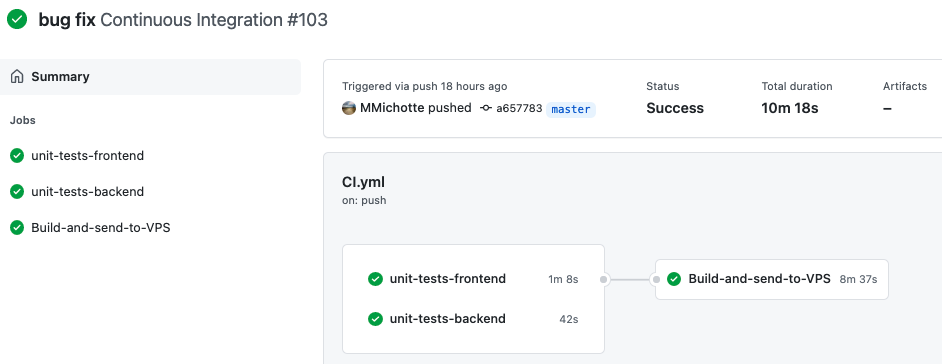
\includegraphics[width=\linewidth]{img/CI-result.png}
  \caption{Exemple résultat du CI/CD}
\end{figure}
